% !TEX root = ../main.tex
\pagebreak[0]
\section{Geometric formulation}\label{sec:geometric-formulation}
\subsection{The rhombicosidodecahedron}\label{subsec:the-rhombicosidodecahedron}

The RID is an Archimedean solid: all its faces are regular polygons---20
equilateral triangles, 30 squares and 12 regular pentagons---and it is
\emph{vertex-transitive}, meaning that its symmetries can carry any vertex
to any other. At each of its 60 vertices, the faces meet in the order
triangle, square, pentagon, square; altogether it has 120 edges
\citep{McCooeyRID}. It has icosahedral symmetry, which we will use to reduce
the configuration domain in \cref{sec:symmetry-reduced-domain}.

For the calculations, we need exact coordinates. The golden ratio
$\varphi=(1+\sqrt5)/2$, familiar from regular pentagons, makes these
particularly simple. Let $V$ consist of all
independent sign choices and cyclic coordinate permutations of
\begin{equation}\label{eq:rhombicosidodecahedron-vertices}
  (1,1,\varphi^3),\qquad
  (\varphi^2,\varphi,2\varphi),\qquad
  (2+\varphi,0,\varphi^2).
\end{equation}
Here cyclic permutation means replacing $(a,b,c)$ by $(b,c,a)$ or $(c,a,b)$.
The three families contain respectively 24, 24 and 12 distinct points,
giving the 60 vertices. Their convex hull, which we denote by $\mathcal R$, is the
filled RID with edge length two; these are also the coordinates used by
\citet{SteiningerYurkevich2023}.
Using edge length two keeps the coordinates simple. Rescaling both the plug
and hole by the same factor does not change whether they fit.

The sign choices make $V=-V$ and hence $\mathcal R=-\mathcal R$, expressing central symmetry
about the origin. The first family includes the eight corners of
$[-1,1]\times[-1,1]\times[-\varphi^3,\varphi^3]$, so the origin lies in
the interior of $\mathcal R$. This will let us compare the two shadows from a common
interior point.

The shape also appears outside polyhedral geometry: a modified RID forms
the connector balls in Zometool.\footnote{The author's childhood experience
of building with Zometool provided an additional motivation for choosing
the RID.} In the connector's idealized polyhedral model, the triangular
faces have edges $\varphi$ times as long as those of the pentagonal faces,
and rectangles with this same side ratio replace the squares
\citep[pp.~51, 197]{HartPicciotto2001}.

The golden ratio is present throughout this geometry: the 1,770 pairs of
vertices lie at 17 distinct distances, and all but two of their squares are
irrational numbers of the form $a+b\sqrt5$; the two exceptions are the
edge and the diagonal of a square face.

At unit edge length, the regular RID has volume
$(60+29\sqrt5)/3\approx41.6153$ \citep{McCooeyRID}, which rounds to 42.\footnote{Also
the answer to life, the universe and everything in \emph{The Hitchhiker's
Guide to the Galaxy} \citep{Adams1979}.}

\subsection{Projection containment}\label{subsec:projection-containment}

Fix a vector $\mathbf u\in\mathbb R^3\setminus\{\mathbf0\}$ along the direction
of motion. Orthogonal projection onto the plane $\mathbf u^\perp$ is the map
$\pi_{\mathbf u}:\mathbb R^3\to\mathbf u^\perp$ defined by
\[
  \pi_{\mathbf u}(\mathbf v)
    =\mathbf v-\frac{\mathbf v\cdot\mathbf u}{\mathbf u\cdot\mathbf u}\mathbf u.
\]
The image of a body under this map is its \emph{shadow}, including the
interior; the boundary of the shadow is its \emph{silhouette}. Since the
projection is linear, the shadow of $\mathcal R$ is the convex hull of the projected
vertices $\pi_{\mathbf u}(\mathbf v)$, for $\mathbf v\in V$.

Suppose initially that the hole is $R_{H}\mathcal R$ and the plug is $R_{P}\mathcal R+\mathbf a$, where
$R_{H},R_{P}\in\operatorname{SO}(3)$ are their rotations about the origin and
$\mathbf a\in\mathbb R^3$ is a displacement. Here $\operatorname{SO}(3)$ is
the group of real $3\times3$ orthogonal matrices with determinant $1$. Translating
the plug along $\mathbf u$ does not change its shadow. Over the whole line of motion,
the plug sweeps out the cylinder consisting of all lines parallel to $\mathbf u$ through
its shadow. The plug can pass through the hole with positive clearance,
giving a fit configuration, exactly when
\begin{equation}\label{eq:strict-projection-containment}
  \pi_{\mathbf u}(R_{P}\mathcal R)+\pi_{\mathbf u}(\mathbf a)
    \subseteq\operatorname{int}_{\mathbf u^\perp}\pi_{\mathbf u}(R_{H}\mathcal R),
\end{equation}
where the interior is taken in the two-dimensional screen plane
\citep[Proposition~1]{SteiningerYurkevich2023}.
Indeed, strict containment leaves room for a slightly wider cross-section
around the plug's shadow, still inside the hole's shadow, so the plug can
move through with positive clearance. Conversely, a fit requires the
entire plug shadow to lie in the interior of the hole shadow.
This is also called a \emph{strict fit}; without qualification, fit always
has this meaning.
A \emph{weak fit} requires only ordinary containment, allowing the plug's
shadow to meet the boundary of the hole's shadow. Such contact is permitted
but not required, so weak fit includes both fit and touch configurations.
Displacement along $\mathbf u$ only changes the plug's starting position, so only
the planar displacement $\pi_{\mathbf u}(\mathbf a)$ enters this comparison.

\paragraph{Removing translations.}
For centrally symmetric bodies, the planar displacement can be discarded.
The following short argument is the centering reduction of
\citet[Proposition~2]{SteiningerYurkevich2023}; it applies equally to weak fit
and to a uniformly scaled plug.

\begin{lemma}[Centering]\label{lem:centering}
  Let $P=-P$ and $H=-H$ be convex planar bodies centred at the origin.
  If a translate $P+\mathbf b$ is contained in $H$, then $P$ is contained in $H$.
  If $P+\mathbf b$ is contained in $\operatorname{int}H$, then $P$ is contained in
  $\operatorname{int}H$.
\end{lemma}
\begin{proof}
  Reflecting $P+\mathbf b\subseteq H$ through the origin gives $P-\mathbf b\subseteq H$.
  For each $\mathbf p\in P$, the points $\mathbf p+\mathbf b$ and $\mathbf p-\mathbf b$ belong to $H$, so their
  midpoint $\mathbf p$ belongs to $H$ by convexity. The same argument works in
  $\operatorname{int}H$, which is also convex and centrally symmetric.
\end{proof}

Both projected copies of $\mathcal R$ are centrally symmetric. Thus, for any fixed
orientations and viewing direction, a translated fit exists exactly when
the centred plug fits. Replacing $P$ by $\lambda P$ in
\cref{lem:centering} gives the same conclusion for each scale $\lambda>0$.
We may consequently restrict the search, and the optimization of scale, to
coincident projected centres. A displacement can still turn a fit configuration
into a touch or poke configuration; the reduction preserves the
existence of a fit.

\paragraph{Fixing the hole.}
Finally, rotating the whole configuration by $R_{H}^{-1}$ fixes the hole as $\mathcal R$
and replaces the plug rotation by $R_{H}^{-1}R_{P}$, with the viewing direction
rotated along with them. In this fixed-hole frame, we continue to write
$\mathbf u$ for the viewing vector and $R_{P}$ for the plug's rotation.
From now on, a configuration $c$ is centred and
consists of a viewing line together with the plug's rotation relative to
this fixed hole. The respective hole and plug shadows are:
\[
  H_c=\pi_{\mathbf u}(\mathcal R),\qquad P_c=\pi_{\mathbf u}(R_{P}\mathcal R).
\]
The sign and length of $\mathbf u$ do not matter: only its line matters. We are left
with two degrees of freedom for the viewing direction and three for the
relative rotation. For a polyhedron that is not centrally symmetric, the
component of the plug's displacement relative to the hole perpendicular
to the viewing direction must generally also be retained. This adds two
degrees of freedom, giving seven in total.

\subsection{Parametrisation of the configuration space}\label{subsec:parametrisation-of-the-configuration-space}

We choose coordinates that make the projected vertices rational functions
of five real parameters. This will allow us to compare their positions using
polynomial inequalities that we verify with exact arithmetic. We represent
the viewing line by a vector with positive $z$-coordinate, scaled to
\[
  \mathbf u=(s,t,1),\qquad (s,t)\in\mathbb R^2.
\]
Thus $s$ and $t$ determine the viewing line. The RID has sufficiently many symmetries
that we can choose such a representative with bounded $s,t$, without needing
any viewing direction in the $xy$-plane. We prove this reduction in
\cref{sec:symmetry-reduced-domain}.

\paragraph{Relative rotation.}
For the relative rotation, we use a nonzero quaternion
$q=(\alpha,\mathbf a)\ne(0,\mathbf0)$, consisting of a scalar part
$\alpha\in\mathbb R$ and a vector part $\mathbf a\in\mathbb R^3$.
We write $\lVert\cdot\rVert$ for Euclidean length.
A rotation by angle $\theta\in[0,\pi]$ around an axis
$\mathbf n\in\mathbb R^3$ with $\lVert\mathbf n\rVert=1$ is
represented by the unit quaternion
\[
  q=(\alpha,\mathbf a)=(\cos(\theta/2),\mathbf n\sin(\theta/2)).
\]
Here $\alpha^2+\lVert\mathbf a\rVert^2=1$. Nonzero real scalar multiples
represent the same rotation. Whenever $\alpha\ne0$, we may
therefore divide by it and write
\[
  q=(1,\mathbf r),\qquad
  \mathbf r=\frac{\mathbf a}{\alpha}=(r_1,r_2,r_3)\in\mathbb R^3.
\]
The vector $\mathbf r$ is a coordinate for the rotation, not the rotation
itself. For $\mathbf r\ne\mathbf 0$, its direction is the rotation axis and its
length is $\tan(\theta/2)$ for the angle $0<\theta<\pi$. The corresponding rotation
acts on a spatial vector $\mathbf v$ by
\begin{equation}\label{eq:relative-rotation}
  R_{P}(\mathbf r)\mathbf v
  =\frac{(1-\mathbf r\cdot\mathbf r)\mathbf v
      +2\mathbf r(\mathbf r\cdot\mathbf v)+2\mathbf r\times\mathbf v}
     {1+\mathbf r\cdot\mathbf r}.
\end{equation}
For example, the component parallel to $\mathbf r$ stays fixed; on the
perpendicular plane the two coefficients are
$(1-\lVert\mathbf r\rVert^2)/(1+\lVert\mathbf r\rVert^2)=\cos\theta$
and $2\lVert\mathbf r\rVert/(1+\lVert\mathbf r\rVert^2)=\sin\theta$.
This verifies the axis and angle and fixes the sign of the rotation.
At $\mathbf r=\mathbf 0$ the formula gives the identity matrix. In this
fixed-hole frame, a configuration is aligned exactly when the relative
rotation is a symmetry of $\mathcal R$.
We will denote a configuration by
$c=[s,t,\mathbf r]\in\mathbb R^2\times\mathbb R^3$, or equivalently
$[s,t,(r_1,r_2,r_3)]\in\mathbb R^5$, wherever these
coordinates are available.

\begin{figure}[htbp]
\centering
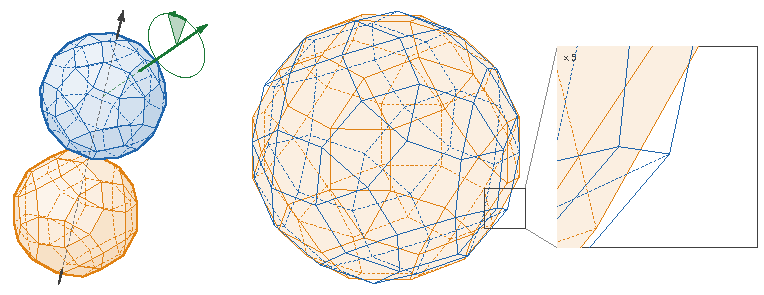
\includegraphics[width=0.78\linewidth]{figures/rid-parametrisation}
\caption{A configuration $c=[s,t,\mathbf r]$ with $s=1/5$, $t=1/10$ and $\mathbf r=(1/4,-1/12,5/24)$. Left: \fc{Hole}{the hole (orange)} and \fc{Plug}{the plug (blue)}, moved apart along the viewing direction $\mathbf u=(s,t,1)$ (black arrow) so that both can be seen. The plug is turned about \fc{Normal}{the axis $\mathbf n=\mathbf r/\lVert\mathbf r\rVert$ (green arrow, from the plug's centre) by the angle $\theta=2\arctan\lVert\mathbf r\rVert\approx37^\circ$, shaded on a circle about the axis}; dashed lines run behind or inside the solids. Middle: the two shadows along $\mathbf u$. Right: the plug's shadow sticks out of the hole's (enlarged five times), so this configuration is a poke.}
\label{fig:rid-parametrisation}
\end{figure}

\paragraph{Screen coordinates.}
There is a similarly simple choice of coordinates on the screen. Define
$L_{s,t}:\mathbb R^3\to\mathbb R^2$ by
\begin{equation}\label{eq:screen-map}
  L_{s,t}(v_1,v_2,v_3)=(v_1-sv_3,\ v_2-tv_3).
\end{equation}
Its kernel is precisely the viewing line spanned by $\mathbf u=(s,t,1)$.
Consequently, its restriction $T$ to $\mathbf u^\perp$ is an invertible linear map
from that plane to $\mathbb R^2$, and
$L_{s,t}=T\pi_{\mathbf u}$. In other words, it gives coordinates for the same
orthogonal shadow. Although these coordinates can distort lengths and
angles, applying the same invertible map to both shadows preserves
containment and containment in the interior. It also commutes with uniform
scaling, so every comparison of a scaled plug shadow with the hole shadow
is preserved.

Using these screen coordinates, we can write the hole and plug shadows as:
\begin{equation}\label{eq:shadow-coordinates}
  H_c=L_{s,t}\mathcal R
      =\operatorname{conv}\{L_{s,t}\mathbf v:\mathbf v\in V\},\qquad
  P_c=L_{s,t}R_{P}(\mathbf r)\mathcal R
      =\operatorname{conv}\{L_{s,t}R_{P}(\mathbf r)\mathbf v:\mathbf v\in V\}.
\end{equation}
Projected hole vertices have coordinates affine in $s,t$, while projected
plug vertices have rational coordinates with the common denominator
$d=1+\lVert\mathbf r\rVert^2\ge1$. Their coefficients belong to the quadratic field
\[
  \mathbb Q(\sqrt5)=\{a+b\sqrt5:a,b\in\mathbb Q\},
\]
because the vertices have coordinates in this field. Each coefficient is
represented exactly by the two rational numbers $a$ and $b$. Multiplying a
comparison by $d$, or by a positive power of $d$, preserves its sign.
This is how the rational expressions give polynomial inequalities without
requiring bounds on trigonometric or other transcendental functions.
The parameters themselves remain real;
the field describes the coefficients of these expressions.

This parametrisation does not represent rotations by $180^\circ$
(half-turns), whose representing quaternions have scalar part zero.
The reduction in \cref{sec:symmetry-reduced-domain} also provides bounded
relative-rotation representatives, including for these rotations.
Until that reduction is proved, a statement
about all configurations refers to the geometric configurations of
\cref{subsec:projection-containment}, not merely those represented by
these parameters.

\subsection{The margin function and \emph{fit} / \emph{poke} / \emph{touch}}\label{subsec:the-margin-function-and-fit-poke-touch}

To measure how close a configuration is to fitting, we compare the two
shadows on rays from their common origin. This gives a relative scale:
we ask how far the plug shadow extends compared with the hole shadow,
rather than measuring an absolute distance between their silhouettes.

For a compact convex shadow $C$ containing the origin in its interior and
a unit planar vector $\boldsymbol{\omega}$, define its \emph{radial extent} by
\[
  \rho_C(\boldsymbol{\omega})=\max\{\lambda\in\mathbb R_{\ge0}:\lambda\boldsymbol{\omega}\in C\}.
\]
Each ray meets $C$ in exactly the segment from the origin to
$\rho_C(\boldsymbol{\omega})\boldsymbol{\omega}$. This extent is positive and finite, and it varies
continuously with $\boldsymbol{\omega}$. To see the continuity, a limit of ray endpoints
still belongs to $C$, by compactness. In the other direction, any point
strictly between the origin and an endpoint is interior, by convexity and
the interior disk about zero; a small change of direction keeps that point
inside. Together these observations prevent either an upward or a downward
jump in radial extent.

\begin{definition}[Configuration margin]\label{def:configuration-margin}
  For a centred configuration $c$, with hole shadow $H_c$ and plug shadow
  $P_c$, define
  \begin{equation}\label{eq:configuration-margin}
    M_{\mathcal R}(c)=\max_{\lVert\boldsymbol{\omega}\rVert=1}
      \frac{\rho_{P_c}(\boldsymbol{\omega})}{\rho_{H_c}(\boldsymbol{\omega})}.
  \end{equation}
\end{definition}
The maximum exists because the unit circle is compact and the denominator
is positive. The largest ratio controls containment of the whole shadow:
it is the smallest factor by which the hole shadow must be scaled to
contain the plug shadow.

\begin{figure}[htbp]
\centering
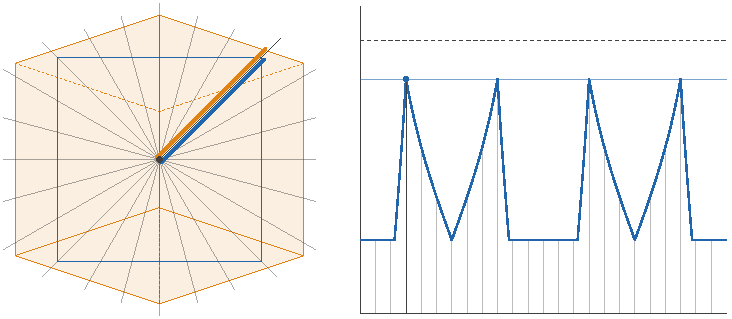
\includegraphics[width=0.78\linewidth]{figures/margin}
\caption{The margin of two congruent cubes $\mathcal C$ in the orientations of \cref{fig:nieuwland-cube}. Left: \fc{Hole}{the hole's shadow (orange)} and \fc{Plug}{the plug's (blue)} about their common centre, with rays every $15^\circ$; along the ray where the plug's radial extent is largest relative to the hole's, the two extents are drawn side by side. Right: that ratio over a full turn of directions, the \fc{Grey}{grey lines} marking the rays on the left. Its maximum, marked, is the margin $M_{\mathcal C}(c)=2\sqrt2/3\approx0.943$; it lies below the dashed level~$1$, so $c$ is a fit.}
\label{fig:margin}
\end{figure}

\begin{lemma}[Margin and containment]\label{lem:margin-and-containment}
  For every centred configuration $c$ and every $\lambda\in\mathbb R_{>0}$,
  \[
    P_c\subseteq\lambda H_c \quad\Longleftrightarrow\quad M_{\mathcal R}(c)\le\lambda,
    \qquad
    P_c\subseteq\operatorname{int}(\lambda H_c)
      \quad\Longleftrightarrow\quad M_{\mathcal R}(c)<\lambda.
  \]
  The margin is unchanged by applying the same invertible linear screen
  map to both shadows.
\end{lemma}
\begin{proof}
  Containment holds exactly when the plug shadow's radial extent is at most
  $\lambda$ times the hole shadow's in every direction. For interior
  containment, every radial comparison is strict. Since the maximum ratio
  is attained, these comparisons are equivalent to $M_{\mathcal R}(c)<\lambda$.
  Finally, an invertible linear map preserves each relation
  $P_c\subseteq\lambda H_c$, and hence preserves the least possible $\lambda$.
\end{proof}

In particular, the rational screen of \cref{eq:screen-map} gives the same
margin as orthogonal screen coordinates. We can now express the three
configuration types introduced in \cref{sec:introduction} as predicates:
\begin{equation}\label{eq:fit-poke-touch}
  \begin{aligned}
    \operatorname{fit}(c)   &\quad\Longleftrightarrow\quad M_{\mathcal R}(c)<1,\\
    \operatorname{touch}(c) &\quad\Longleftrightarrow\quad M_{\mathcal R}(c)=1,\\
    \operatorname{poke}(c)  &\quad\Longleftrightarrow\quad M_{\mathcal R}(c)>1.
  \end{aligned}
\end{equation}
A touch configuration has a weak fit with at least one boundary point shared by the two shadows. In the direction
from the common origin to such a point, the radial extents of the hole and
plug shadows match. In particular,
aligned configurations have identical shadows and margin one,
since their radial extents match for all $\boldsymbol{\omega}$.
Note that the silhouettes do not necessarily have to fully coincide in
a touch configuration.

\paragraph{Scale and the Nieuwland number.}
Scaling the plug by $\lambda>0$ multiplies every numerator in
\cref{eq:configuration-margin} by $\lambda$. It fits weakly exactly when
$\lambda M_{\mathcal R}(c)\le1$, and strictly exactly when $\lambda M_{\mathcal R}(c)<1$.
Thus $1/M_{\mathcal R}(c)$ is the maximum scale for weak fit and the supremum of the
scales for strict fit.

\emph{Optimising the margin over the full configuration space means taking
its infimum, which is the reciprocal of the Nieuwland number}
\citep[Definition~3]{SteiningerYurkevich2023}:
\begin{equation}\label{eq:nieuwland-number-and-margin}
  \nu(\mathcal R)=\sup_c\frac{1}{M_{\mathcal R}(c)}
        =\frac{1}{\inf_c M_{\mathcal R}(c)}.
\end{equation}
Here $c$ ranges over all centred geometric configurations. The centering
lemma shows that allowing translations does not improve this supremum.
It is finite: if $\mathcal R$ contains a ball of radius $a>0$ and is contained in
one of radius $b$, both centred at zero, then the orthogonal shadows contain
radius-$a$ disks and lie in radius-$b$ disks, giving
$a/b\le M_{\mathcal R}(c)\le b/a$. Aligned configurations give $\nu(\mathcal R)\ge1$.
Consequently \emph{$\mathcal R$ is Rupert exactly when $\nu(\mathcal R)>1$, and Nopert exactly
when $\nu(\mathcal R)=1$}. A barely Rupert body has a best margin just below one,
or equivalently a Nieuwland number just above one.

The examples in \cref{subsec:previous-approaches-and-the-remaining-difficulty}
show how little clearance known fit configurations can have. For the triakis
tetrahedron, \citet{Fredriksson2024} reported a lower bound of $1.000004$,
which \citet{GosainGrimmer2025V1} refined numerically to $1.000004055715$,
still only about four parts per million above one.
For Tom~7's candidate~\#214, the Lean formalisation of
\citet{RenshawRupertLean} proves fit,
and its accompanying source reports a shadow clearance of approximately
$1.8\times10^{-8}$ in the published coordinate units
\citep{Renshaw2026Nopert214Video,RenshawRupertLean}.
This last value measures a distance rather than a scale factor.

\paragraph{Continuity of the margin.}
After the compact
representative domain is established in \cref{sec:symmetry-reduced-domain},
continuity will also justify attaining the minimum margin there.

A useful geometric picture is that small changes to a configuration produce
small changes to its margin, even when the choice of projected vertices and
edges forming the silhouette changes discontinuously. For example, a projected
vertex can move onto or away from the boundary as the viewing direction
changes, while the shadow and its margin continue to vary continuously.

\begin{proposition}\label{prop:continuity-and-openness}
  The margin $M_{\mathcal R}$ is continuous on centred configurations. The sets of
  fit and poke configurations are open, and the set of touch configurations
  is closed.
\end{proposition}
\begin{proof}
  Work near any given configuration. Choose fixed spatial axes so that
  the viewing line has a representative with positive $z$-coordinate, and use the rational
  screen \cref{eq:screen-map} throughout a neighbourhood. Let the entries
  of the actual relative rotation matrix vary continuously; this includes
  half-turns. Each projected vertex then varies continuously, whether or
  not it lies on the silhouette.

  Compare configurations $c$ and $c'$, and let $\delta$ be the largest
  displacement between corresponding projected vertices of either body.
  Every point of a shadow is a convex combination of its projected
  vertices. Keeping the same coefficients in the other configuration gives
  a point within distance $\delta$, in both directions.
  All four shadows contain a common disk of some radius $a>0$ about zero:
  $\mathcal R$ and its rotations contain a radius-$a$ ball, and
  $L_{s,t}(v_1,v_2,0)=(v_1,v_2)$.

  Put $\lambda=1+\delta/a$. For any corresponding pair of shadows $C,C'$,
  the preceding distance bound implies $C\subseteq\lambda C'$.
  Indeed, write a point of $C$ as $\mathbf p+\mathbf z$, with $\mathbf p\in C'$ and
  $\lVert\mathbf z\rVert\le\delta$. If $\delta>0$, then
  \[
    \frac{\mathbf p+\mathbf z}{\lambda}
      =\frac{1}{\lambda}\mathbf p+
        \frac{\delta/a}{\lambda}\frac{a}{\delta}\mathbf z
      \in C'
  \]
  by convexity and the interior disk; if $\delta=0$, the inclusion is
  immediate. The reverse inclusion $C'\subseteq\lambda C$ follows in the
  same way. One factor of $\lambda$ compares the plug shadows and another
  compares the hole shadows:
  \[
    P_{c'}\subseteq\lambda P_c
      \subseteq\lambda M_{\mathcal R}(c)H_c
      \subseteq\lambda^2M_{\mathcal R}(c)H_{c'}.
  \]
  Using \cref{lem:margin-and-containment} and then reversing the roles of
  $c$ and $c'$ gives
  \[
    \lambda^{-2}M_{\mathcal R}(c)\le M_{\mathcal R}(c')\le\lambda^2M_{\mathcal R}(c).
  \]
  As $c'$ tends to $c$, the finitely many vertex displacements tend to
  zero, so $\lambda$ tends to one. This proves continuity. The openness
  and closedness statements follow from the comparisons with one in
  \cref{eq:fit-poke-touch}.
\end{proof}
